\section{引言}
\label{sec:introduction}
面对一个由图像生成的三维消防车，观察者可以轻易指出车轮、车门和云梯；对于下游程序，这个资产却可能只是一组带纹理的三角面。生成质量的提高使模型更像一个完整物体，但没有自动给出“哪一片表面属于哪个部件”的解释。部件级检索、局部选择与交互展示不仅需要几何外观，还需要把可解释的部件身份关联到空间区域。图\ref{fig:motivation}以概念示意说明了这一差别。

二维可提示分割提供了一条利用图像理解三维结构的途径：先在渲染图中提取部件，再将二维引导输入三维模型。困难在于，自动候选掩码通常依据视觉可分性产生，不一定符合任务所需的语义粒度。一个连贯的大区域可能覆盖多个功能部件，而若干细碎区域也可能只是同一部件的纹理变化。另一方面，逐个框选和修正部件需要人工介入，难以直接扩展到大量生成资产。这里缺少的不是单纯“更多掩码”，而是把部件意图转化为可靠空间约束的过程。

视觉语言模型能够描述可见部件，但名称本身不能替代分割。将“车轮”作为一条文本记录保存，不会自动改变 SAM2 的边界，也不会使三维输出具备稳定的语义 ID。本文采取显式接口：让 Qwen3-VL 同时提出部件名称、边界框和正负点，以空间提示驱动冻结的 SAM2；再通过候选级反馈和点引导融合生成二维部件图，作为冻结 SegViGen 的输入。名称随部件记录保留，语言通过空间提示影响分割，而非被未经验证地注入三维隐空间。

这一接口面临两个具体问题。首先，首次提示可能定位不准，多个正点或负点也可能相互冲突，因此需要依据候选掩码的可见结果进行有限反馈。其次，多个部件的掩码可能重叠，若大区域先覆盖，小件会在融合阶段消失。本文分别采用每个候选至多一次的视觉反馈，以及清理后的小框优先仲裁处理这两类问题，同时记录无效候选和失败回退，保留从名称到二维区域的可追溯关系。

本文的工作由三部分构成。第一，组织一条不重新训练基础模型的视觉语言引导流水线，将英文部件规划、空间提示和三维分割接口明确分离。第二，实现候选反馈与点引导的小框优先融合，并保存二维整数标签、调色板及部件记录，使分割变化能够追溯到具体提示与处理阶段。第三，建立面向生成资产的分层评价方案，分别考察二维引导、最终三维输出的可见表面、人工多视图判断和运行成本。本文不以输出区域数量或 SAM2 自预测分数代替真实评价；各模块能否提高最终质量，将由同一测试集合上的主实验与消融结果验证。

\begin{figure*}[t]
  \centering
  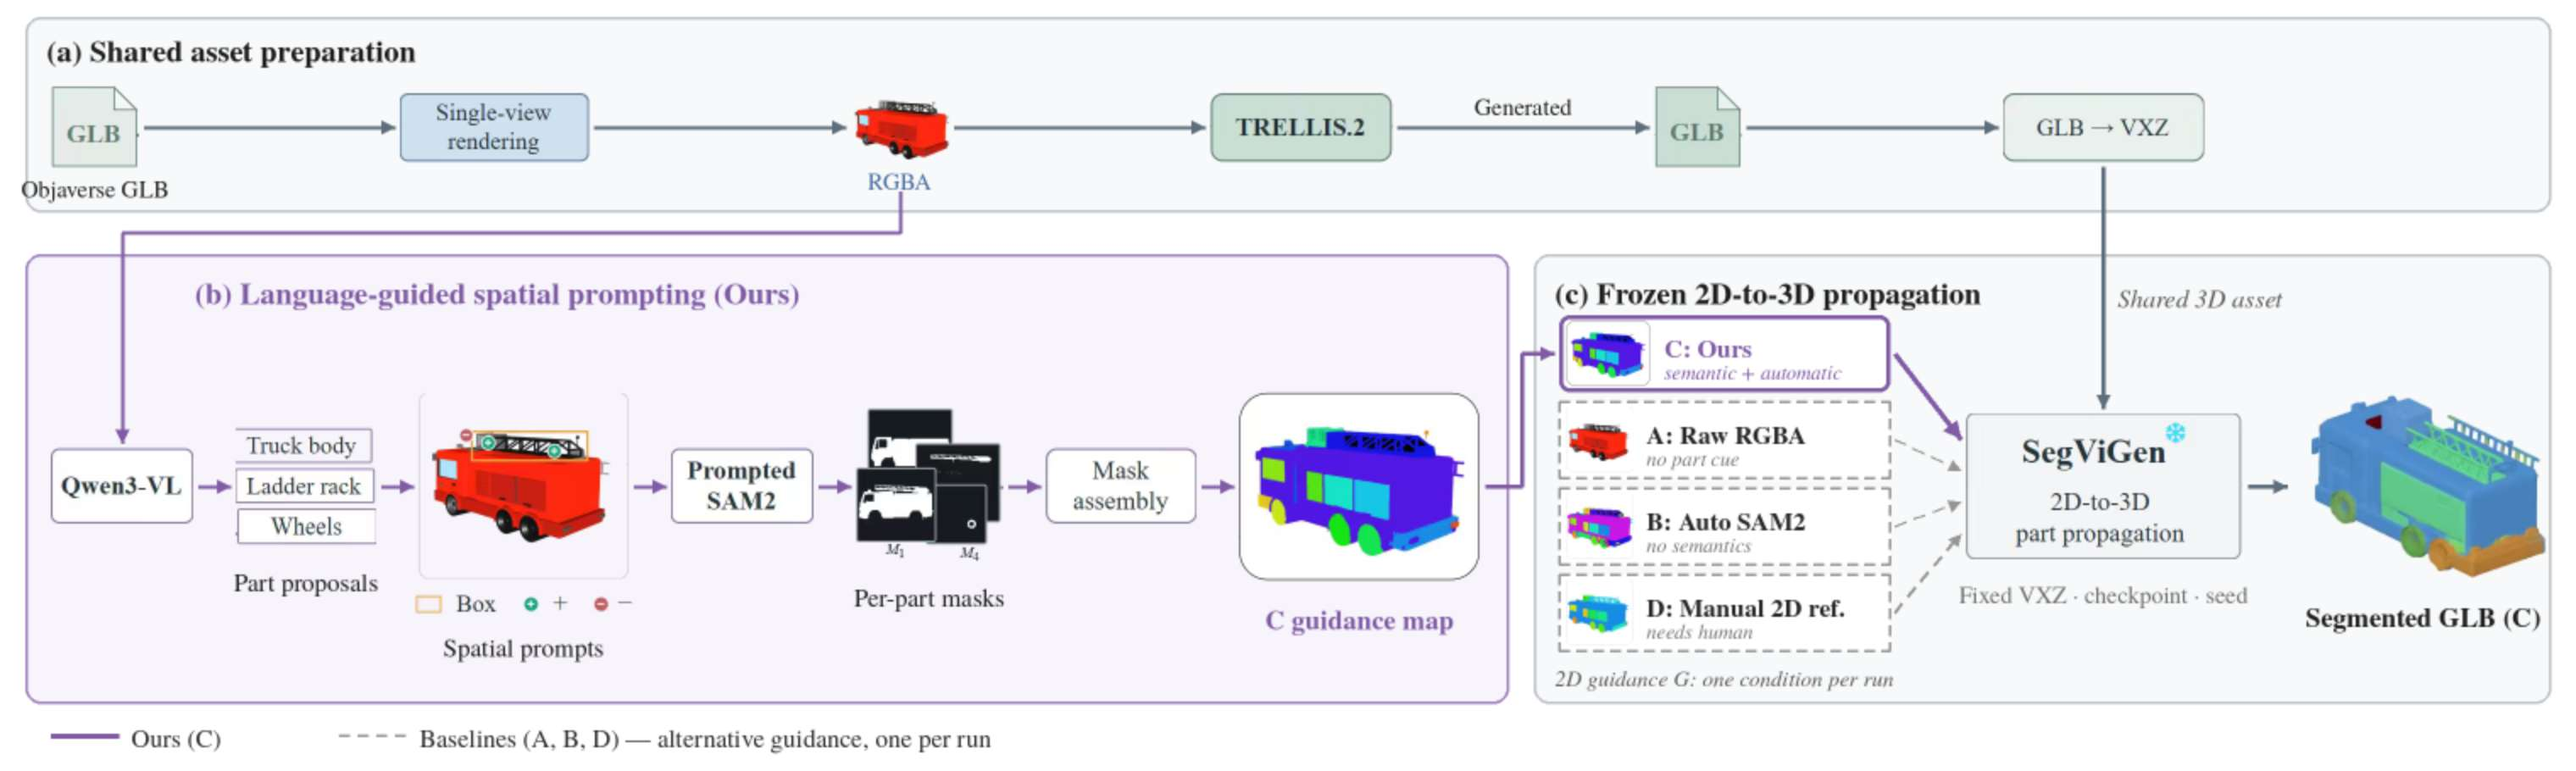
\includegraphics[width=\textwidth]{images/fig1_method.jpg}
  \caption{方法概览。（a）由下载的三维资产渲染输入图像，并构建供比较实验使用的生成资产；（b）Qwen3-VL 提出可见部件及空间提示，SAM2 生成候选掩码，经反馈与融合得到 C 组二维引导；（c）在固定三维资产和推理设置下，每次仅输入一种引导条件，由 SegViGen 输出三维部件分区。A、B、D 是替代引导条件，不与 C 同时输入。图中 ``Shared'' 描述本文采用的受控比较协议，不代表不同条件的最终分割 GLB 相同。候选反馈的具体位置见图\ref{fig:data}。}
  \label{fig:method}
\end{figure*}

